\documentclass{classrep}
\usepackage[utf8]{inputenc}
\usepackage{color}
\usepackage{graphicx}
\usepackage{amsmath}
\usepackage{amssymb}

\DeclareUnicodeCharacter{00A0}{~}

\studycycle{Informatyka, studia dzienne, inż I st.}
\coursesemester{IV}

\coursename{Sztuczna inteligencja i systemy ekspertowe}
\courseyear{2022/2023}

\courseteacher{Krzysztof Lichy}
\coursegroup{poniedziałek, 12:15}

\author{
  \studentinfo{Amadeusz Sitnicki}{242524} \and
  \studentinfo{Artur Surosz}{242542}
}

\title{Zadanie 2: Poprawa lokalizacji UWB przy pomocy sieci neuronowej}

\begin{document}
\maketitle


\section{Cel}
{
Celem wykonania zadania jest zapoznanie się z działaniem sieci neuronowych i technik uczenia maszynowego poprzez stworzenie programu, który dokonuje poprawy współrzędnych wyznaczonych przez zewnętrzny system, tak aby zmniejszyć błędy w wyznaczanej przez niego lokalizacji. W celu weryfikacji działania sieci konieczna jest wizualizacja danych w postaci wykresów dystrybuanty rozkładu błędu zarówno poprawianej lokalizacji wyznaczonej przez zewnętrzny system \ppauza jak i poprawionej lokalizacji wyznaczonej przez wytrenowany model uczenia maszynowego. }

\section{Wprowadzenie}
{
Przy rozwijaniu algorytmów sztucznej inteligencji, twórca modelu matematycznego często wzoruje się na zjawiskach zachodzących naturalnie w biologii.
W przypadku sieci neuronowych \ppauza model ten próbuje naśladować \ppauza i w pewnym stopniu odwierciedla reakcje mające miejsce w układzie nerwowym organizmów żywych. 
    \begin{figure}[!htbp]
            \centering
            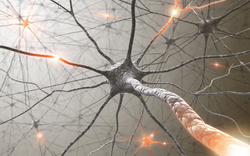
\includegraphics[width=\textwidth, width=90mm]{neural_biolo.jpg}
            \caption{Ilustracyjny obraz układu nerwowego organizmów żywych}
            \label{neural_biolo}
    \end{figure}
 Jako model matematyczny sieć neuronowa jest kolekcją skłądającą się z :
    \begin{itemize}
            \item Warstwy danych wejściowych
	\item Pewnej liczby warstw neuronów pośredniczących - tzw. warstwy ukryte
	\item Warstwy neuronów wyjściowych
           
    \end{itemize}
Graficznie można przedstawić przykładową sieć neuronową przy pomocy diagramu zamieszczonego na ilustracji.
    \begin{figure}[!htbp]
            \centering
            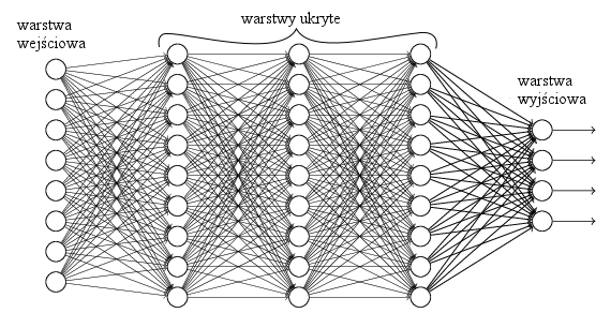
\includegraphics[width=\textwidth, width=150mm]{neuro_mat.png}
            \caption{Diagram ilustrujący model sieci neuronowej}
            \label{neuro_mat}
    \end{figure}
Każde połączenie posiada przyporządkowaną wagę. Każdy neuron przetwarza dane w następujący sposób: 
     \begin{itemize}
            \item Dla każdego połączenia przychodzącego odbierana jest wartość wejściowa
	\item Każda z wartości wejściowych wymnażana jest przez wagę danego połączenia
	\item Obliczana jest ważona suma wartości wejściowych
           \item Obliczana jest wartość nieliniowej funkcji aktywacji neuronu dla ważonej sumy wartości wejściowych
           \item Wartość funkcji aktywacji jest przekazywana dalej jako wartość wyjściowa neuronu
           
      \end{itemize}

Jeśli sieć neuronowa posiada $k_{we}$ wejść $x_i$, ${k_{wy}}$ neuronów wyjściowych o wagach $w_{nij}$, funkcji aktywacji $f_n(x)$ i wartościach wyjściowych $o_i$ oraz $n$ warstw ukrytych o liczebnościach $l_i$ z neuronami o wagach $w_{ijk}$ oraz funkcjach aktywacji $f_{i}$ o wartościach wyjściowych $h_{ij}$ , to:
    \begin{itemize}
            \item $h_{0i} = f_0(\sum_{j=0}^{k_{we}} w_{0ij}x_{j})$
	\item $h_{i+1, k} =f_i(\sum_{k=0}^{l_i} w_{ijk}h_{ik}) $
	\item $o_i = f_n(\sum_{j=0}^{k_{wy}} w_{nij} h_{n-1, j})$ 
      \end{itemize}
}
Aby sieć realizowała powierzone jej zadania, należy tak dobrać wartości wag sieci, aby określona funkcja straty dla sieci osiągnęła jak najmniejszą wartość.
Funkcja straty może mieć następującą postać:
$$L(\vec{w}) = \frac{1}{m} \sum_{i=1}^{m} (o_i-d_i)^2, $$ gdzie $d_i$ są pożądanymi wartościami wyjść sieci neuronowej z kolekcji m przykładowych danych dla sieci. Takie przykładowe dane dla sieci, które służą ustalaniu wag połączeń w sieci neuronowej noszą nazwę zbioru treningowego. 

Dobór wag połączeń w sieci neuronowej jest równoważny zagadnieniu optymalizacji funkcji straty $L(\vec{w})$, która jest określona na przestrzeni o tylu wymiarach, ile jest połączeń w sieci neuronowej. Zatem funkcja straty jest odwzorowaniem: $$L: \mathbb{R}^{k_{we} l_0 +\sum_{i=0}^{n-2} l_i l_{i+1} + l_{n-1}k_{wy}} \mapsto \mathbb{R}.$$

W naszym rozwiązaniu użyjemy metody stochastycznego zejścia gradientowego (SGD) w celu stopniowego aktualizowania wartości wag i obniżania funkcji straty.
Ciąg aktualizacji wag jest określony przez wzór rekurencyjny:
$$\vec{w}_{i+1} = \vec{w_i} + \vec{\nabla}L(\vec{w_i})$$ 

Wartości pochodnych cząstkowych $\frac{\partial L}{\partial w_i}$ można obliczać dzięki zdefiniowaniu pewnego zbioru liczbowego:
Uogólniony zbiór liczb dualnych rzędu $r$ określamy jako zbiór liczb rzeczywistych rozszerzony o obiekty $\varepsilon_i$, $i=1,2,...,r.$
Obiekty $\varepsilon_{i}$ spełniać muszą dwie zależności:
    \begin{itemize}
            \item $\varepsilon_{i} \varepsilon_{j} = 0$
	\item  $\varepsilon_{i} \notin \mathbb{R} \land  \varepsilon_{j} \notin \mathbb{R}$ 
      \end{itemize}

Na podstawie tej definicji da się udowodnić, że:
$$L(\vec{w}+\vec{\varepsilon}) = L(\vec{w}) + \sum_{i=1}^{r} \varepsilon_{i} \frac{\partial L}{\partial w_i} = L(\vec{w}) + \vec{\varepsilon} \cdot \vec{\nabla}L(\vec{w})$$
Powyższa równość pozwala na bezpośrednie wyznaczanie gradientu funkcji straty wprost z definicji tej funkcji i nietrudnej w implementacji arytmetyki na uogólnionych liczbach dualnych.

\section{Opis implementacji}
{
Program realizujący oraz trenujący sieć neuronową został stworzony na potrzeby zajęć laboratoryjnych przy pomocy języka C++ oraz kompilatora MinGW-W64 g++ 12.2.0 jako aplikacja konsolowa uruchamiana z poziomu wiersza poleceń powłoki systemowej. Implementacja sieci neuronowej od podstaw z trenowaniem w oparciu o uogólnione liczby dualne. 
    \begin{figure}[!htbp]
            \centering
            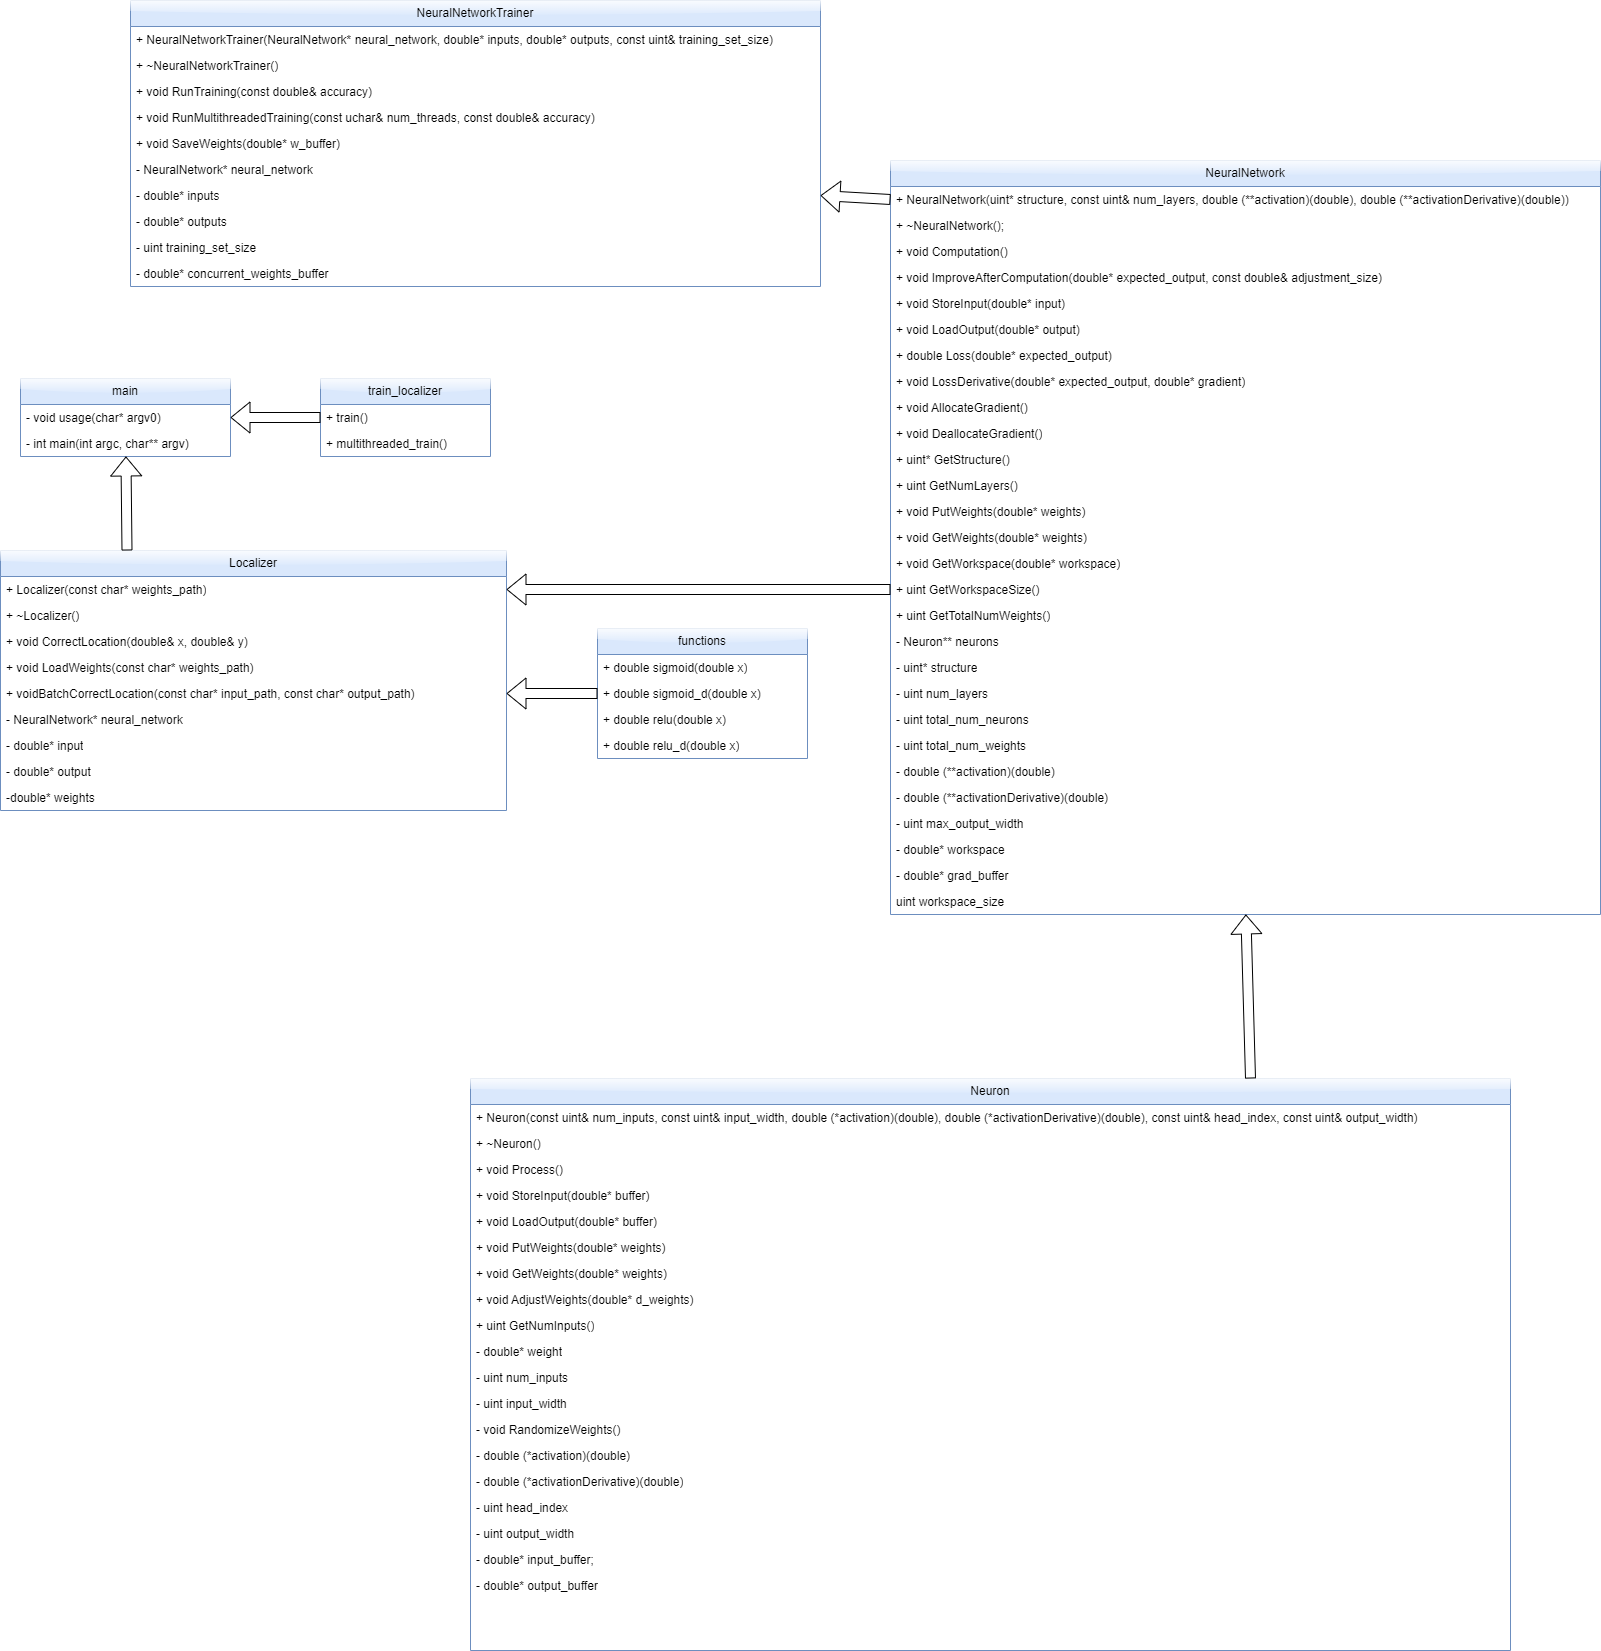
\includegraphics[width=\textwidth, width=150mm]{loca.png}
            \caption{Schemat powiązań plików i klas rozwiązania C++}
            \label{loca}
    \end{figure}

Program pomocniczy wizualizujący dystrybuanty rozkładów błędu lokalizacji wyznaczonej przez system a także służący do ekstrakcji danych m. in. z plików xlsx, napisany został przy użyciu języka Python oraz ogólnodostępnych bibliotek.

    \begin{figure}[!htbp]
            \centering
            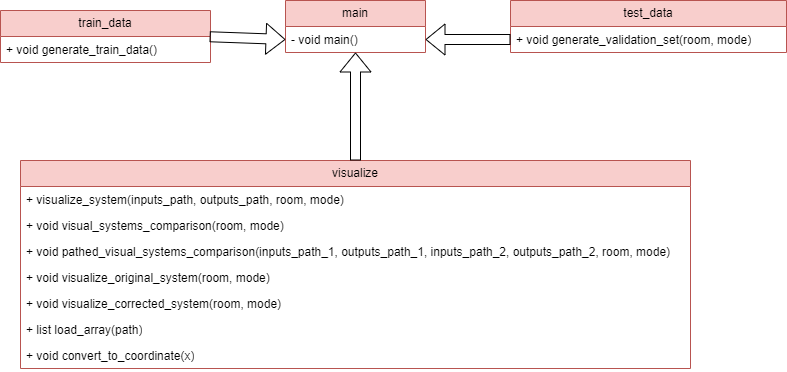
\includegraphics[width=\textwidth, width=150mm]{locapyth.png}
            \caption{Schemat powiązań plików rozwiązania Python}
            \label{locpyth}
    \end{figure} 
}

\section{Materiały i metody}
{
	W celu wytrenowania sieci neuronowej:
	 \begin{itemize}
            	\item {} Ekstrakcja danych z plików .xlsx \ppauza wykonanie poniższych poleceń języka Python, odwołując się do pomocniczych skryptów test\_data.py oraz train\_data.py :			\linebreak\linebreak 
			generate\_train\_data() \linebreak
    			generate\_validation\_set\text{("f8", "1p")} \linebreak
			generate\_validation\_set\text{("f8", "1z")} \linebreak
			generate\_validation\_set\text{("f8", "2p")} \linebreak
			generate\_validation\_set\text{("f8", "2z")} \linebreak
			generate\_validation\_set\text{("f8", "3p")} \linebreak
			generate\_validation\_set\text{("f8", "3z")} \linebreak
			generate\_validation\_set\text{("f10", "1p")} \linebreak
			generate\_validation\_set\text{("f10", "1z")} \linebreak
			generate\_validation\_set\text{("f10", "2p")} \linebreak
			generate\_validation\_set\text{("f10", "2z") }\linebreak
			generate\_validation\_set\text{("f10", "3p")} \linebreak
			generate\_validation\_set\text{("f10", "3z")} \linebreak
			generate\_validation\_set\text{("f8", "random\_1p")} \linebreak
			generate\_validation\_set\text{("f8", "random\_2p") }\linebreak
			generate\_validation\_set\text{("f10", "random\_1p") }\linebreak
			generate\_validation\_set\text{("f10", "random\_2p") }\linebreak
            	\item {} Uruchomienie procesu trenującego sieć (wagi zapisywane są w katalogu weights):
			\linebreak\linebreak
			$...\backslash$localizer$\backslash >$loca train 
			
            	\item {} Po zakończeniu trenowania uruchomienie procesu wykonawczego sieci neuronowej dla wybranego pliku z wagami:
			\linebreak\linebreak
			$...\backslash$localizer$\backslash >$loca run weights$\backslash$weights\_0\_00428953.bin

		\item {} Wizualizacja dystrybuant obu rozkładów błędów (przed i po filtrowaniu SN) \ppauza wykonanie poniższych poleceń języka Python, odwołując się do pomocniczego skryptu visualize.py:
			\linebreak\linebreak
			visual\_systems\_comparison\text{("f8", "1p")} \linebreak
			visual\_systems\_comparison\text{("f8", "1z")}\linebreak
			visual\_systems\_comparison\text{("f8", "2p")}\linebreak
		           visual\_systems\_comparison\text{("f8", "2z")} \linebreak
			visual\_systems\_comparison\text{("f8", "3p")} \linebreak
			visual\_systems\_comparison\text{("f8", "3z")} \linebreak
			visual\_systems\_comparison\text{("f10", "1p"}) \linebreak
			visual\_systems\_comparison\text{("f10", "1z")} \linebreak
			visual\_systems\_comparison\text{("f10", "2p")} \linebreak
			visual\_systems\_comparison\text{("f10", "2z")} \linebreak
			visual\_systems\_comparison\text{("f10", "3p")} \linebreak
			visual\_systems\_comparison\text{("f10", "3z")} \linebreak
			visual\_systems\_comparison\text{("f8", "random\_1p")} \linebreak
			visual\_systems\_comparison\text{("f8", "random\_2p")} \linebreak
			visual\_systems\_comparison\text{("f10", "random\_1p")} \linebreak
			visual\_systems\_comparison\text{("f10", "random\_2p")} \linebreak
           \end{itemize} 
}

\section{Wyniki}
{
	Zaprojektowana i zrealizowana sieć neuronowa posiada:
	\begin{itemize}
	          \item 2 wejścia
           	\item 4 warstwy neuronowe
                     \item liczebności warstw neuronowych to odpowiednio 20, 10, 5, 2
                     \item sieć posiada 2 neurony wyjściowe
                     \item dla każdego neuronu funkcja aktywacji ustalona jest jako funkcja sigmoidalna $\sigma (x) = -1+\frac{2}{1+e^{-x}}$ 

           \end{itemize}
      \begin{figure}[!htbp]
            \centering
            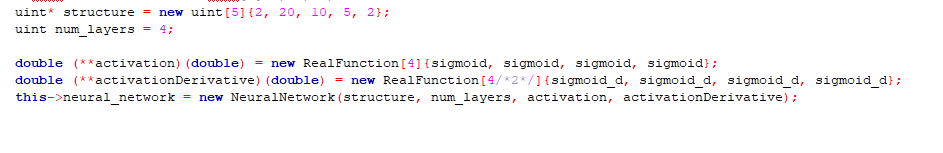
\includegraphics[width=\textwidth, width=150mm]{nn_set.png}
            \caption{Konfiguracja sieci neuronowej w kodzie źródłowym}
            \label{nn_set}
     \end{figure}

        Dodatkowo przed wejściem do sieci, dane podlegają transformacji funkcją:
	$$T(x) = -1+\frac{2}{1+e^{-0.001x}}$$
       Zaś po wyjściu z sieci, dane są przekształcane funkcją odwrotną:
          $$T^{-1}(x) = -1000 \ln (\frac{2}{1+x}-1)$$

      Przypomnijmy, że w naszym rozwiązaniu używamy  metody stochastycznego zejścia gradientowego (SGD) w celu stopniowego aktualizowania wartości wag i obniżania funkcji straty.
      Ciąg aktualizacji wag jest określony przez wzór rekurencyjny:
      $$\vec{w}_{i+1} = \vec{w_i} + \vec{\nabla}L(\vec{w_i})$$ 

      Wartości pochodnych cząstkowych $\frac{\partial L}{\partial w_i}$ można obliczać dzięki zdefiniowaniu pewnego zbioru liczbowego:
      Uogólniony zbiór liczb dualnych rzędu $r$ określamy jako zbiór liczb rzeczywistych rozszerzony o obiekty $\varepsilon_i$, $i=1,2,...,r.$
      Obiekty $\varepsilon_{i}$ spełniać muszą dwie zależności:
    \begin{itemize}
            \item $\varepsilon_{i} \varepsilon_{j} = 0$
	 \item  $\varepsilon_{i} \notin \mathbb{R} \land  \varepsilon_{j} \notin \mathbb{R}$ 
     \end{itemize}

Na podstawie tej definicji da się udowodnić, że:
$$L(\vec{w}+\vec{\varepsilon}) = L(\vec{w}) + \sum_{i=1}^{r} \varepsilon_{i} \frac{\partial L}{\partial w_i} = L(\vec{w}) + \vec{\varepsilon} \cdot \vec{\nabla}L(\vec{w})$$
Powyższa równość pozwala na bezpośrednie wyznaczanie gradientu funkcji straty wprost z definicji tej funkcji i nietrudnej w implementacji arytmetyki na uogólnionych liczbach dualnych.

W wyniku trenowania sieci, minimalna wartość funkcji straty jaką osiągnięto wynosi $L=0.00428953$ 

Na ilustracjach widoczne jest porównanie dystrybuant rozkładu (CDF) błędu lokalizacji \ppauza porównanie dla systemu UWB oraz dla systemu wspomaganego siecią neuronową.

\begin{figure}[!htbp]
            \centering
            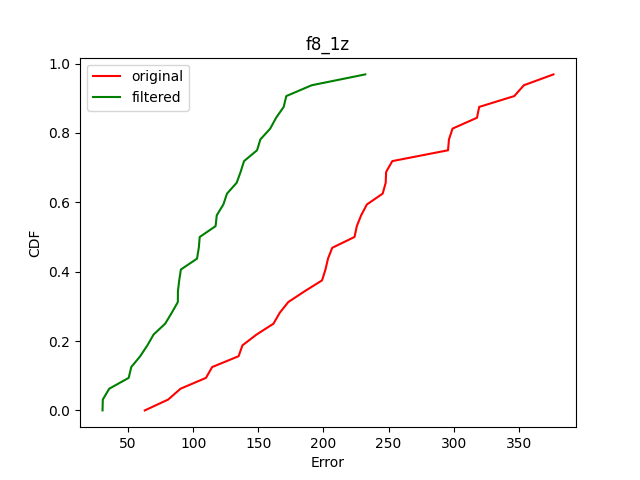
\includegraphics[width=\textwidth, width=90mm]{comparison_f8_1z.png}
            \caption{Porównanie dystrybuant dla f8\_1z}
            \label{comparison_f8_1z}
    \end{figure}

\begin{figure}[!htbp]
            \centering
            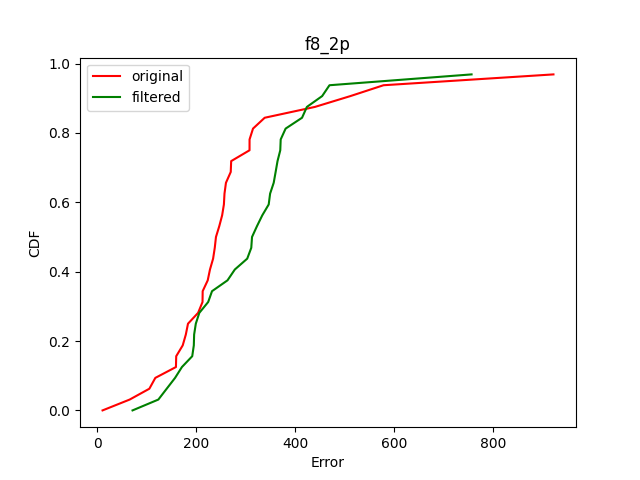
\includegraphics[width=\textwidth, width=90mm]{comparison_f8_2p.png}
            \caption{Porównanie dystrybuant dla f8\_2p}
            \label{comparison_f8_2p}
    \end{figure}

\begin{figure}[!htbp]
            \centering
            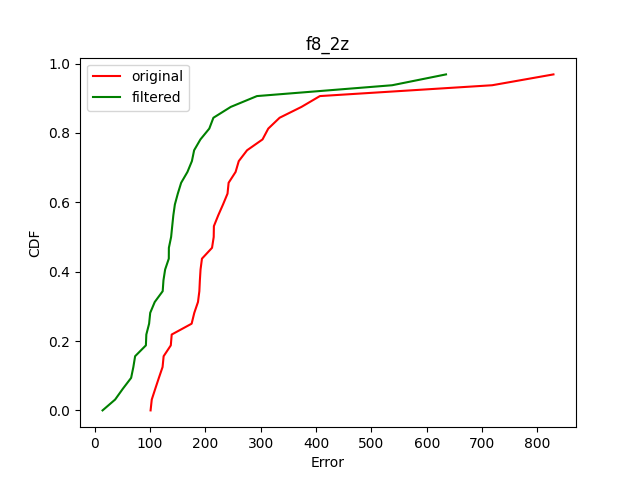
\includegraphics[width=\textwidth, width=90mm]{comparison_f8_2z.png}
            \caption{Porównanie dystrybuant dla f8\_2z}
            \label{comparison_f8_2z}
    \end{figure}

\begin{figure}[!htbp]
            \centering
            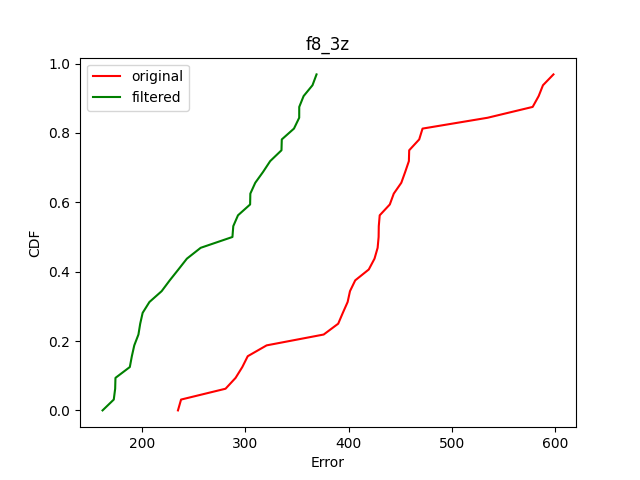
\includegraphics[width=\textwidth, width=90mm]{comparison_f8_3z.png}
            \caption{Porównanie dystrybuant dla f8\_3z}
            \label{comparison_f8_3z}
    \end{figure}

\begin{figure}[!htbp]
            \centering
            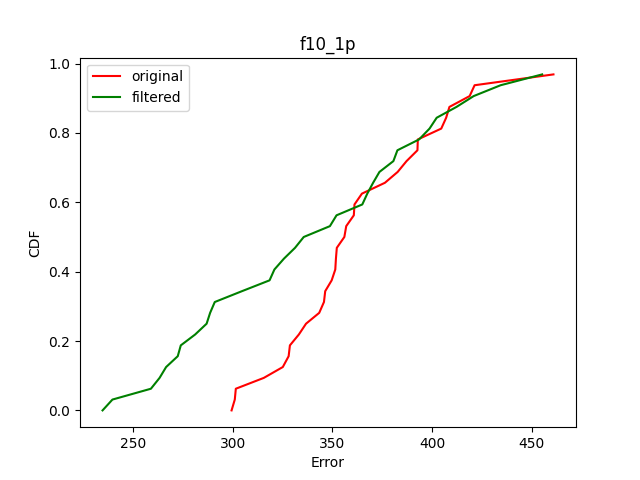
\includegraphics[width=\textwidth, width=90mm]{comparison_f10_1p.png}
            \caption{Porównanie dystrybuant dla f10\_1p}
            \label{comparison_f10_1p}
    \end{figure}

\begin{figure}[!htbp]
            \centering
            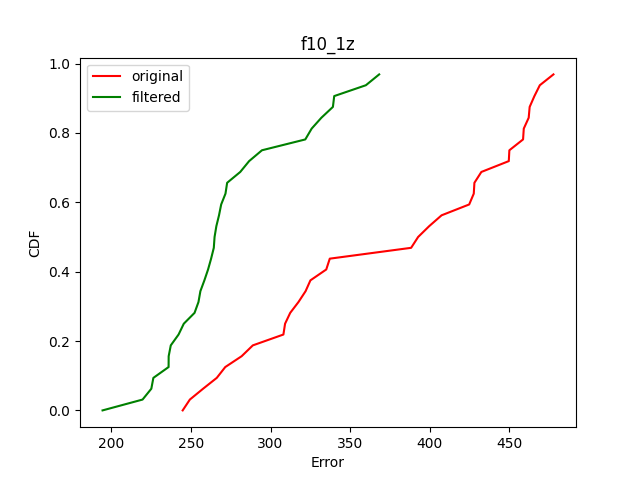
\includegraphics[width=\textwidth, width=90mm]{comparison_f10_1z.png}
            \caption{Porównanie dystrybuant dla f10\_1z}
            \label{comparison_f10_1z}
    \end{figure}

\begin{figure}[!htbp]
            \centering
            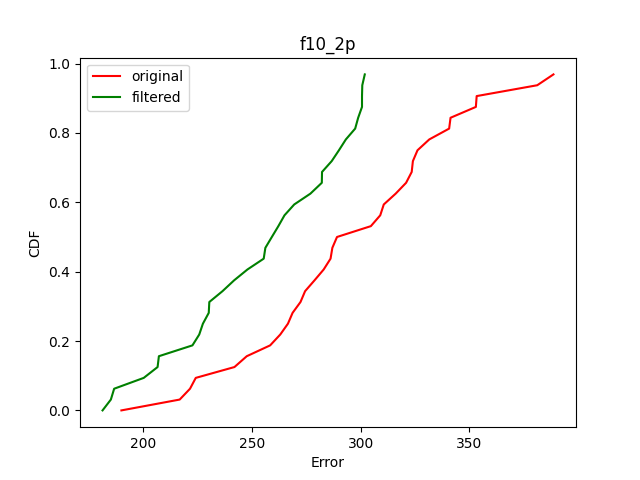
\includegraphics[width=\textwidth, width=90mm]{comparison_f10_2p.png}
            \caption{Porównanie dystrybuant dla f10\_2p}
            \label{comparison_f10_2p}
    \end{figure}

\begin{figure}[!htbp]
            \centering
            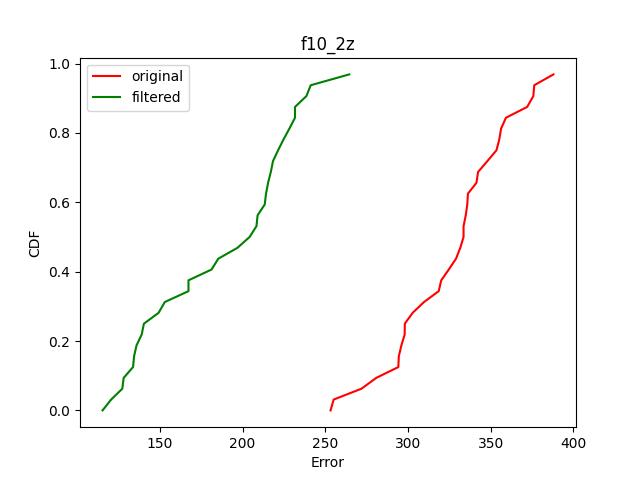
\includegraphics[width=\textwidth, width=90mm]{comparison_f10_2z.png}
            \caption{Porównanie dystrybuant dla f10\_2z}
            \label{comparison_f10_2z}
    \end{figure}

\begin{figure}[!htbp]
            \centering
            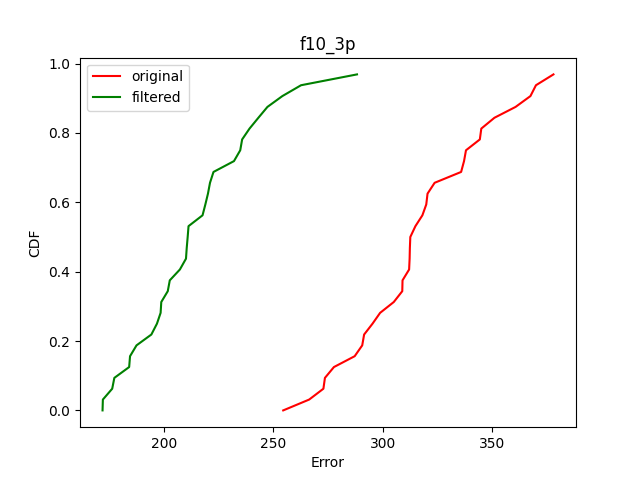
\includegraphics[width=\textwidth, width=90mm]{comparison_f10_3p.png}
            \caption{Porównanie dystrybuant dla f10\_3p}
            \label{comparison_f10_3p}
    \end{figure}

\begin{figure}[!htbp]
            \centering
            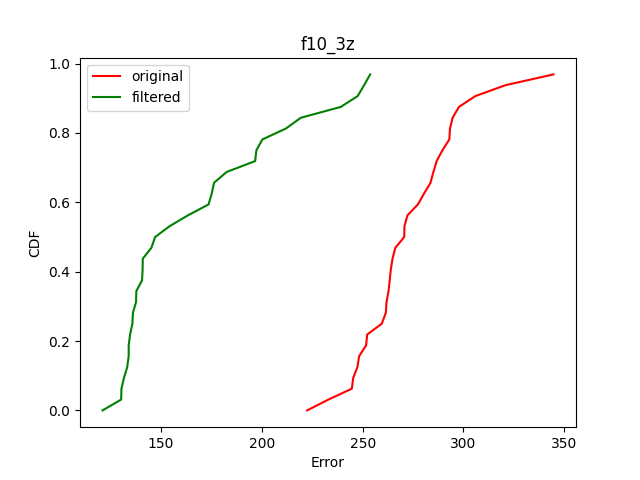
\includegraphics[width=\textwidth, width=90mm]{comparison_f10_3z.png}
            \caption{Porównanie dystrybuant dla f10\_3z}
            \label{comparison_f10_3z}
    \end{figure}

}

\section{Dyskusja}
{
\subsection{Wykorzystana metoda uczenia}{
	Wykorzystana metoda uczenia pozwala wykorzystać własności arytmetyki na uogólnionym zbiorze liczb dualnych. Dzięki temu nie trzeba implementować metody propagacji wstecznej. W ten sposób realizacja zadania jest ułatwiona, a kod \ppauza krótszy, mimo że sieć neuronowa została zaimplementowana od podstaw z wykorzystaniem języka C++.
\subsection{Zrównoleglanie obliczeń}{
	Implementacja algorytmu uczenia sieci w ten sposób ma jednak pewien problem, który polega na gorszym przystosowaniu algorytmu do zrównoleglania. Nie jest jednak wykluczone, że istnieje optymalizacja metody, pozwalająca na zrównoleglenie trenowania modelu \ppauza zbadanie takiego zoptymalizowanego wariantu tej metody pozwoliłoby przywrócić szybkości znajdowania optymalnych wag sieci neuronowej, znane z popularnych bibliotek deep learning wykorzystujących przetwarzanie współbieżne. 
}
\subsection{Skuteczność sieci neuronowej}
	Dla pewnych torów (np. f8\_2p) obliczenia dokonane przez sieć mają mniejszą skuteczność. Możliwe, że taki stan rzeczy jest spowodowany doborem funkcji transformującej dane przed wejściem i po wyjściu z sieci neuronowej - zmienność wartości $T(x)$ (por. rozdział 5) jest w przypadku znajdowania się systemu pomiarowego skrajnie z prawej strony znacząco ograniczona i wykonuje jedynie niewielkie wahania w okolicach wartości 1. Taki efekt może być przyczyna zjawiska i powodować mniejszą skuteczność sieci dla torów ruchu o środku geometrycznym skrajnie z prawej strony obszaru, na którym odbywało się uczenie sieci.
}

\section{Wnioski}
{
\begin{itemize}
	          \item Sieci neuronowe i uczenie maszynowe są bardzo dobrym narzędziem ogólnego przeznaczenia do przewidywania i redukcji błędów pomiarowych
           	\item Skuteczność sieci zależy od systematyczności błędu \ppauza jeśli błąd będzie nosił znamiona losowości osobliwej \ppauza wykrywanie błędów będzie utrudnione 
                     \item Przekształcenia wstępne i końcowe mogą znacząco zaburzyć lub poprawić skuteczność obliczeń przeprowadzanych przez sieć neuronową
                     \item Manipulowanie architekturą sieci, daje szansę na dalsze zmniejszanie funkcji straty, gdy zawiodła wcześniej testowana architektura.
                     \item Nadzorowane uczenie sieci neuronowych jest zadaniem stosunkowo wymagającym obliczeniowo dla sprzętu co wiąże się z wyjątkowo długim czasem oczekiwania przez konstruktora sieci na znalezienie optymalnych parametrów sieci. Pomocą w tej kwestii może być zastosowanie przetwarzania współbieżnego \ppauza najlepiej z użyciem dedykowanych GPU lub jednostek przetwarzających TPU \ppauza szczególnie w przypadku, gdy ma się do czynienia z dużo większymi zbiorami danych niż te obecne w tym projekcie \\ppauza na przykład przetwarzanie obrazów przy użyciu sieci neuronowych.

 \end{itemize}
.}

\begin{thebibliography}{0}
  \bibitem{l2short} 
    \textsl{Sieci neuronowe - Wikipedia}, dostępny
    online.

\bibitem{l2short} T. Oetiker, H. Partl, I. Hyna, E. Schlegl.
    \textsl{Nie za krótkie wprowadzenie do systemu \LaTeX2e}, 2007, dostępny
    online.
\end{thebibliography}

\end{document}
